%%%%% Document Setup %%%%%%%%

\documentclass[10pt, twocolumn]{revtex4}    % Font size (10,11 or 12pt) and column number (one or two).

\usepackage{times}                          % Times New Roman font type

\usepackage[a4paper, left=1.85cm, right=1.85cm,
 top=1.85cm, bottom=1.85cm]{geometry}       % Defines paper size and margin length

\usepackage[font=small,
labelfont=bf]{caption}                      % Defines caption font size as 9pt and caption title bolded


\usepackage{graphics,graphicx,epsfig,ulem}	% Makes sure all graphics works
\usepackage{amsmath} 						% Adds mathematical features for equations

\usepackage{etoolbox}                       % Customise date to preferred format
\makeatletter
\patchcmd{\frontmatter@RRAP@format}{(}{}{}{}
\patchcmd{\frontmatter@RRAP@format}{)}{}{}{}
\renewcommand\Dated@name{}
\makeatother

\usepackage{fancyhdr}
\usepackage{mathtools, diffcoeff}
\DeclarePairedDelimiter\abs{\lvert}{\rvert}
\usepackage{physics}
\usepackage{caption}
\captionsetup{justification=raggedright,singlelinecheck=false}

\pagestyle{fancy}                           % Insert header
\renewcommand{\headrulewidth}{0pt}
\lhead{L. van Schie}                          % Your name
\rhead{Investigation into the Current Carrying Properties of Silicon Germanium via Vegard's Law}            % Your report title               

\def\bibsection{\section*{References}}        % Position refernce section correctly


%%%%% Document %%%%%
\begin{document}


\title{Investigating the Current Carrying Properties of Silicon Germanium via Vegard's Law}
\date{Submitted: \today{}}
\author{Laura van Schie (Supervisor: Dr Halim Kusumaatmaja)}
\affiliation{\normalfont L3 Computing Project, Group C3}

\begin{abstract}

Using methods outlined, this work simulates the band structures of bulk silicon-germanium (or Si$_{1-x}$Ge$_x$) to infer the change in conducting properties with germanium composition of each element. Increasing the proportion of germanium in the compound corresponds to a decrease in the band gap energy. There is a characteristic point at $x$ = 0.8 (proportion of germanium) where the trend in the properties shift, showing a discontinuous transition and giving rise to distinct `silicon-like' and `germanium-like' regimes. The effective mass of electrons in both the longitudinal and transverse directions from the conduction band minima are found. These values agree with literature values in the `silicon' regime but deviate in the `germanium' regime. The effective mass of conduction electrons is then found to be approximately constant with a value of (0.245 $\pm$ 0.005) m$_0$, which is close to the value of the effective mass of silicon, 0.260 m$_0$. A different path of reasoning follows to obtain a relation between electron mobility and composition. The reasons for these discrepancies and the practical applications for these compounds are explored.

\end{abstract}

\maketitle
\thispagestyle{plain} % produces page number for front page



\section{Introduction}


The discovery of semiconductors and their unique current carrying capabilities has ushered in the new era of development known as the `information age'. Their properties can be evaluated physically by examining their band structure. In the ground state the electrons in the lowest energy level exist in what is known as the valence band. The next available energy level corresponding to the first excited state is the conduction band \cite{ref01}.  Semiconductors have a filled valence band and an unfilled conduction band. When electrons are excited to the conduction band they are able to carry negative charge. They leave behind an absence of negative charge known as a `hole' that caries positive charge.\\

Different semiconducting materials (and more specifically their properties) can be distinguished by investigating the topography of the band structure. This is  a plot of the allowed electronic energies as a function of wave vector. By applying the pseudo potential Hamiltonian (that encompasses the energy of a free electron with the potential due to the ions in the lattice of the crystal) to the electron wave function, allowed energies can be found by solving the Schr\"{o}dinger equation,
\begin{equation}
	\frac{-\hbar^{2}}{2me}\nabla^{2}\psi\textsubscript{\textbf{k}}(\textbf{r}) + 	 V(\textbf{r})\psi\textsubscript{\textbf{k}}(\textbf{r}) = E\textsubscript{\textbf{k}} \psi\textsubscript{\textbf{k}}(\textbf{r})
\end{equation}
where $m$ and $e$ represent the mass and charge of the electron respectively, $V(\textbf{r})$ represents the potential energy and $E\textsubscript{\textbf{k}}$ gives the possible energies of the electron.

Electrons in semiconductors are described by Bloch wave functions of the form
\begin{equation}
	\psi\textsubscript{\textbf{k}} = e^{i \textbf{k$\cdot$r}}u\textsubscript{\textbf{k}}
\end{equation}
including a periodic potential term, $u\textsubscript{\textbf{k}}$, to account for periodic perturbations to the electron due to the ions in the lattice. \\


The band structure plot now tells us the properties of the semiconductor. Of interest are the band gap and the curvature. The band gap is the energy gap between the valence and conduction bands that an electron must posses to be excited to the conduction band.
The curvature of the energy surfaces describes the effective mass (that is the apparent mass that an electron can be described as having as it is accelerated by the potential).\\

Pure semiconducting elements are often mixed with other materials to change and optimise their properties. Silicon is commonly used in technology due to its high abundance and resilience in manufacture. Germanium is used in transistors due to its small band gap \cite{ref02}. It has a higher carrier concentration (to the order of 10$^{13}$ cm$^{-3}$) than silicon (10$^{9}$ cm$^{-3}$).  The two are mixed forming compounds that benefit from the higher electron concentration and variable band gap, making them ideal for use in high frequency circuits \cite{ref03}. \\

Mixing of silicon and germanium is similar to normal doping of semiconductors but both have the same number of valence electrons so neither acts as a donor or acceptor. Instead, the transport (scattering) mechanisms in the current change. Both have the same crystal structure (face centred cubic diamond lattices)\cite{ref04} in their pure forms. We can find the properties of the resulting compounds, known as Si$_{1-x}$Ge$_x$ or SiGe by utilizing Vegard's law \cite{ref05}. This states that certain properties of a compound can be found by linearly interpolating the properties of each component in their pure form via the equation \cite{ref06}

\begin{equation}
    \zeta_{SiGe} = (1-x)\cdot\zeta_{Si}  +  x\cdot\zeta_{Ge}
\end{equation}
where $\zeta$ is the property in question, $x$ represents the proportion of germanium and $1-x$ (rather trivially) represents the proportion of silicon. This proportionality can range from 0 to 1 as the lattices are miscible (i.e. form a homogeneous mixture when added together). Silicon and germanium are the only miscible Group IV elements. This method works for bulk SiGe as there is a random array of silicon and germanium ions. In this case the proportionality corresponds to the probability that the electron will interact with each atom.

The linear interpolation is often accepted but usually corrected with a quadratic term known as the bowing parameter
\begin{equation}
    \zeta_{SiGe} = (1-x)\cdot\zeta_{Si}  +  x\cdot\zeta_{Ge} + bx(1-x)
\end{equation}
where $b$ is the bowing parameter. This encompasses experimental disorder that occurs in real crystals that would be absent in a computational case \cite{ref07}.


\section{Methodology}

\subsection{Generating the Band Structure}

To examine the band gap we construct a lattice in reciprocal space rather than real space. In transforming our wave function form real to reciprocal space the face-centred cubic lattice structure and becomes body-centred cubic. The points in this space are described by reciprocal lattice vectors (RLVs) \cite{ref08}. Like in real space, this lattice is periodic and can be described by a repeating pattern known as the first Brillouin zone. Due to the nature of the forces between ions and electrons being Coulombic, interactions between these particles will be inversely proportional to the distance between them. This simplifies the need to generate an infinite sized lattice as we can localise it to where long-ranged forces make a negligible difference.\\

To compute the allowed energies, $E\textsubscript{\textbf{k}}$, we use a matrix refomalisation of  the Schr\"{o}dinger equation \cite{ref09}. This allows us to find the eigenvalues of the matrix, and hence the eigen-energies.
The elements of this matrix are of the form,
\begin{equation}
H_{\textbf{g},\textbf{g'}} = \frac{-\hbar^{2}|\textbf{k} + \textbf{g}|^2}{2me} \delta_{\textbf{g},\textbf{g'}} + 	 V_{\textbf{g} - \textbf{g'}}
\end{equation}

where \textbf{g} and \textbf{g'} represent the position of an RLV in the lattice and \textbf{k} represents the wave vector confined to the Brilloiun zone. The potential term is treated as a perturbation \cite{ref10} so can be found using the pseudopotential form factor method \cite{ref11}. This expands the term in reciprocal lattice vectors. For a face-centred cubic only the symmetric terms are required. They are implemented using the equation
\begin{equation}
V_{\textbf{g} - \textbf{g'}} = V_n cos \left( \frac{a}{8} (\textbf{g} \cdot \mathbf{\tau} )\right)
\end{equation}
where $a$ is the lattice parameter of the material and $\tau$ represents the position of the atom.

The values of the $V_{\textbf{g}}$  are dependant on the magnitude of the reciprocal lattice vector. We follow the method use by Cohen and Bergstreese \cite{ref11} and include the factors where the magnitude of (\textbf{g}$ \cdot \tau$) is 3, 8 \& 11. The nucleons of silicon and germanium have different form factors due to the fact that the nucleons have different atomic masses and charge.\\

Vegard's law is implemented in the lattice parameter, $a$, and the pseudopotential form factors, $V_{\textbf{g}}$. This is achieved by calculating the current carrying features and varying the physical parameters as in \textit{Eqn. 3}.

\subsection{Evaluating the Band Gap}

The band gap is found by taking the difference between the maximum energy of the valence band and the minimum energy of the conduction band. For silicon and germanium (both Group IV elements) the valence band corresponds to the fourth energy level as this is where the valence electron is found. The conduction band is the next highest energy level as this is where the first excited state exists.


The change in energy gap for bulk SiGe is given in \textit{Eqn. 7}.
\begin{equation}
E_{g,SiGe} =
    \begin{cases}
      1.17 - 0.47x + 0.24x^2, & \text{x \textless \  0.85}\\
      5.88 - 9.58x + 4.43x^2, & \text{x \textgreater \ 0.85}\\
    \end{cases}
\end{equation}

This is in tandem with experimental evidence \cite{ref12}. The change in trend at $x$ = 0.85 is due to the band gap going from being `silicon-like' to  `germanium-like.' \\


The errors have been calculated using the quoted errors for constants from NIST. As the form factors have been estimated they have not been quoted with a value for error. Instead this is evaluated by deviating the form factors by one digit in the lowest decimal place and finding the change this has on the band gap. The difference between this and the obtained band gap is the absolute error.

\subsection{Finding the Effective Mass of Charge Carriers}

The effective mass of the charge carrying electrons can be found by finding the curvature of the conduction band as this is where the electrons are promoted to and become mobile.
The change in momentum of the electron in a crystal is proportional to the external force. Characterising the derivative in reciprocal space (\textbf{k}) rather than real space (\textbf{r}) gives us the equation for the effective mass of the electron, \cite{ref13}
\begin{equation}
m^* = \hbar^2 \left[ \frac{d^2E}{dk_i dk_j}\right]^{-1}
\end{equation}
where $i,j$ represent the direction of the k wave vector. \\


As the minimum of the conduction band is not centred at the origin, the resulting energy surface around this point  is anisotropic in different directions for both silicon and germanium. Due to this anisotropy the effective mass has a longitudinal component, $m_l$, in the direction of the band extremum and a transverse component, $m_t$, at right angles to this. We therefore find the position of this extremum point and generate the band in the transverse direction to find both components of effective mass. \\

As we cannot analytically find the derivative from the generated values for the energy in the band structure we use the method of finite difference. The formula for the second order derivative using the central finite difference method is given by \cite{ref14}
\begin{equation}
\left(\pdv[2]{E}{k_i}\right)_{\ }=\ \frac{E_{m+1}-2E_m+E_{m-1}}{\left(\Delta k_i\right)^2}+\mathcal{O}\left(\Delta k_i\right)^2
\end{equation}

%\begin{equation}
%\left(\pdv{^2E}{k_i k_j}\right)_{\ }=\ \frac{E_{m+1,n+1}-E_{m-1,n+1}-E_{m+1,n-1}+E_{m-1,n-1}}{4\Delta k_i \Delta k_j}+\mathcal{O}[\left(\Delta k_i\right)^2 \left(\Delta k_j\right)^2
%\end{equation}
where $m$ represents the position of the minimum in the $i$ or $j$ direction.
The error is the truncated error $\mathcal{O}\left(\Delta k_i\right)^2$. The derivative is then used in \textit{Eqn. 8} and the the effective mass components are calculated.\\

The effective mass of conduction electrons can be calculated via the equation
\begin{equation}
m^*_e = \frac{3}{\frac{1}{m_l}+\frac{2}{m_t}}.
\end{equation}

This better describes the mobility of conduction electrons as we can intuitively infer that a lower effective mass will correspond to a higher mobility.



\section{Results and Analysis}

\subsection{Numerical Convergence}

The table below demonstrates the convergence of the results to a value for the band gap in silicon (1.089 eV) using an increasing number of reciprocal lattice vectors (RLVs). The results are compared to the percentage error this deviation would result in for the value of energy gap. We generate 113 lattice vectors as for this amount the band gap changes by less than 1\% and hence the result has converged to a suitable degree.\\

\begin{table}[h!]
\begin{tabular}{|c|c|c|}
\cline{1-3}
\textbf{Number of RLVs} & \textbf{Difference in band gap} &  \textbf{\% Error} \\ \cline{1-3}
9              & -                     &-  \\ %\cline{1-3}
15             & 2.890           & 259.0 \\ %\cline{1-3}
27             & 0.578             & 53.1 \\ %\cline{1-3}
51             & 0.026            & 2.43 \\ %\cline{1-3}
59             & 0.081            & 7.40 \\ %\cline{1-3}
65             & 0.015           & 1.32 \\ %\cline{1-3}
89             & 0.017            & 1.68 \\ %\cline{1-3}
113            & 0.016             &  1.54\\ %\cline{1-3}
137            & 0.0015018             & 0.20 \\ \cline{1-3}

\end{tabular}
\caption{A table illustrating the convergence of the value for the band gap as the number of RLVs used increases. The error calculated from the computationally derived band gap is included to demonstrate its minimisation.}

\end{table}
The band is described in 100 steps up to the boundary of the first Brillioun zone, i.e where  $|\textbf{k}| = \frac{2\pi}{a}$. The number of steps was derived in a similar fashion to the number of reciprocal lattice vectors, but using a linearly increasing number of steps. As an arbitrary number of steps can be used and in the interest of being economic with space, the results have not been illustrated here.
The proportion of germanium was changed in steps of 0.05 from 0 to 1.  This is sufficient to analyse and identify the key points in the trend in both effective mass and band gap.


\subsection{Noting the Change in Topology of the Band Structure.}

The change in the topology of the valence and conduction bands is shown in \textit{Fig. 1}.
\begin{figure}[h!]
 \hspace*{-0.5cm}
  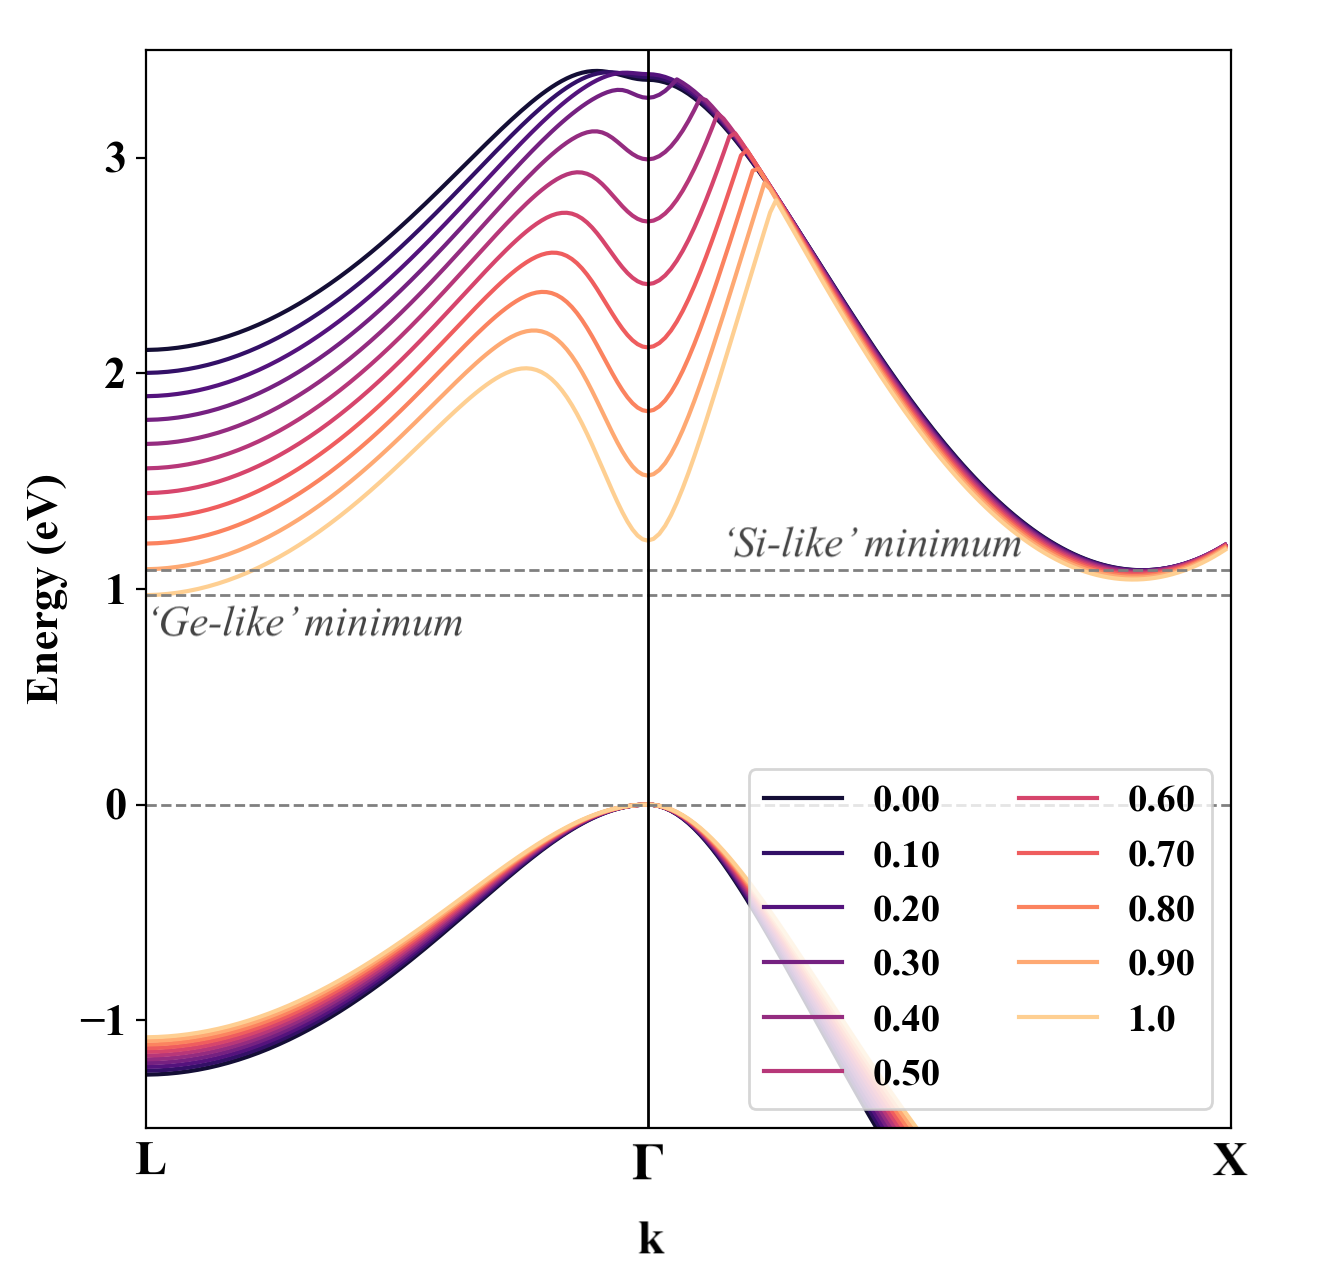
\includegraphics[width=260pt,height=260pt]{bands.png}

    \caption{Valence and Conduction Bands of SiGe compounds in the X and L-directions. The legend identifies the fractional composition of germanium in each compound. The valence band maximum and conduction band minima in both the X (silicon) and L (germanium) directions have been labelled. }
\end{figure}

There is a more drastic change in the band structure in the L-direction (i.e. the wave vector corresponds to \textbf{k} = $\frac{2\pi}{a} (1,1,0)$) than in the X-direction (\textbf{k} = $\frac{2\pi}{a} (1,1,0)$) due to the potential in this direction being stronger. These strong perturbations allow us to lower the band gap by increasing the germanium proportion as intended. The shape of the conduction band is what dictates the changes in the band gap as the shape of the valence band does not deviate appreciably at the point of the maximum. This implies that deviations in current carrying characteristics are due to chages in first excited state and not the ground state. Increasing the composition of germanium also has the consequence of lowering the direct band gap \cite{ref15}.\\

As will become more clear in Section III.C we also need to consider the change in energy in transverse direction at the point of the minimum. \textit{Fig. 2} illustrates the energy surface in two dimensions, as the second transverse dimension will be symmetric to the first \cite{ref16}. The constant energy surfaces of the conduction band for various compositions have been plotted to illustrate the change in the curvature with germanium composition.
\begin{figure}[h!]
 \hspace*{-0.5cm}
  \includegraphics[width=260pt,height=230pt]{cont.png}

    \caption{Energy surface of various compositions of silicon germanium. The fractional composition of germanium in each case has been indicated. Yellow corresponds to higher energies; purple corresponds to lower energies. The conduction band minima have been labelled with a white `x' in each case.}
\end{figure}

This demonstrates once again the shift in minima and the the anisotropy of the change in energy surface in each direction.

\subsection{Analysing the Trend in Band Gap with Germanium Composition}

A plot of the minimum band gap energy and the compositional fraction of germanium is illustrated in \textit{Fig. 3}.
\begin{figure}[h!]
 \hspace*{-0.5cm}
  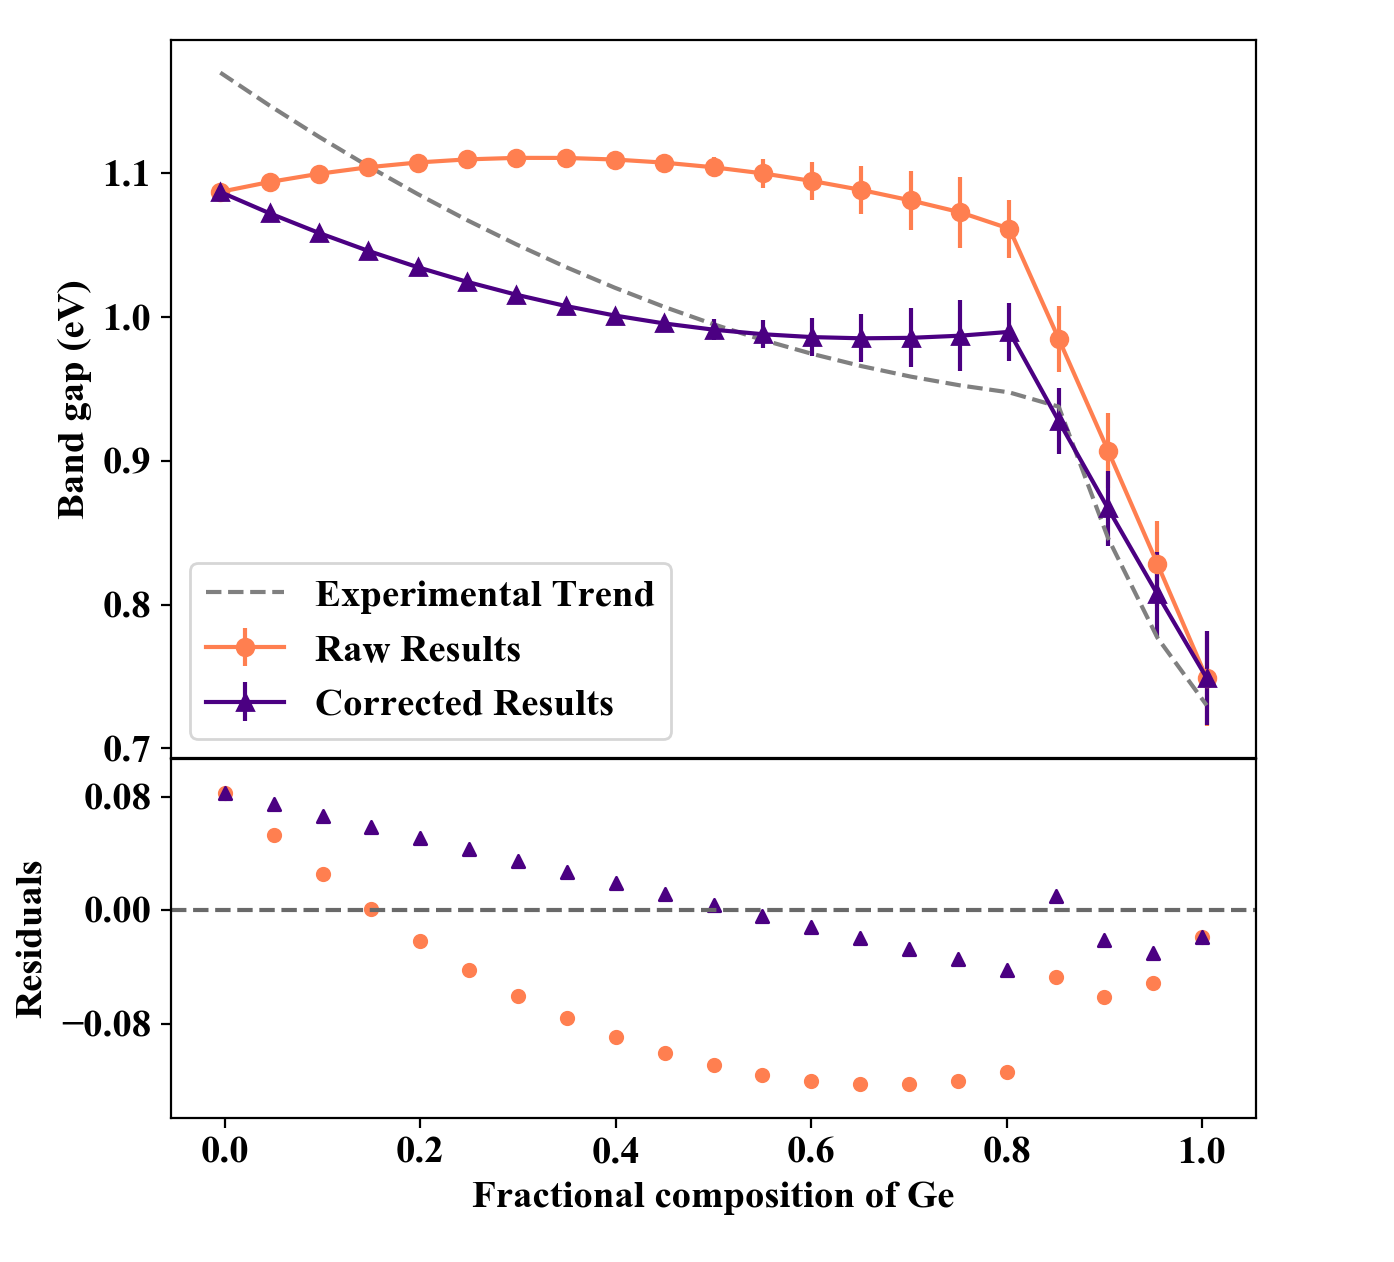
\includegraphics[width=260pt,height=250pt]{bg.png}

    \caption{Variation of band gap with composition of germanium. Experimental values from Weber \& Alonso \cite{ref12} have been included for comparison. Both the original results (orange) and the results corrected with the trial bowing parameter (purple) have been included. Raw residuals have been plotted.}
\end{figure}

This shows a decrease in the size of the band gap with an increase in the proportion of germanium. There is a sharp change in the trend for the band gap at a fractional composition of 0.80 germanium. Here the compound is said to go from being `silicon-like' (as the conduction band minimum is in the same location as for silicon) to become `germanium-like' (as the conduction band minimum is now found where it is characteristic to find it in germanium). We shall call the minimum in the `silicon-like' phase the X-minimum and in the `germanium-like phase' the L-minimum. Due to symmetry the conduction band minimum is six-fold degenerate in the silicon-like regime and eight-fold degenerate in the germanium-like regime. \\

Comparison with the given experimental results from Weber \& Alonso \cite{ref12} shows a disagreement in the shape of the trend. The turning point is delayed to 0.85 in the literature. This variation is possibly because the form factors used have over-estimated the strength of the germanium interaction in mixing. We notice further inconsistency in the results from 0.80 $< x <$ 1 (germanium-like regime) where the results differ from experimental results without a clear trend.\\

We have derived a negative quadratic trend, where a positive quadratic is expected. This, with the quadratic shape of the residuals,implies that correction via the bowing parameter may be necessary. Although the bowing parameter can easily be applied to the lattice parameter \cite{ref05} as this is expected to change linearly, correcting the pseudopotential form factors is not as simple due to the lack of trend between form factors. \\

Instead we find the band gap of the composition by directly apply the bowing parameter to these relations as it is suggested that this property obeys Vegard's law. We take note of the discontinuity by supposing that the linear interpolation works for the band gap at a specific point (X and L-minima) and not the smallest possible band gap, allowing us to combine the two trends for the final result. This will be of the form \cite{ref18}
\begin{equation}
E_{g,SiGe} =
    \begin{cases}
      (1-x) E_{Si,X}  +  xE_{Ge,X} + bx(1-x), & \text{x \textless \  0.85}\\
      (1-x) E_{Si,L}  +  x E_{Ge,L} + bx(1-x) & \text{x \textgreater \ 0.85}\\
    \end{cases}
\end{equation}
where the subscripts, $X \& L$ denote the location of the band gap.\\

The literature suggests a bowing parameter of $b$ = -0.0273 \cite{ref04}. By fitting the residuals with a second order polynomial fit we use the quadratic term as the bowing parameter. We add each of these bowing parameters to the `silicon-like' and germanium-like' trends to correct the results, as in \textit{Eqn. 4}. \\

The goodness of fit has been evaluated using reduced chi-squared. The results are summarised in \textit{Table II} \cite{ref12}.
\begin{table}[h!]
\begin{tabular}{|l|c|c|}
\hline
             & \textbf{Bowing Parameter} &$ \mathbf{\chi^2_{min}}$\\ \hline
\textbf{No Correction}       & -                & 2.01     \\
\textbf{Literature Bowing Parameter}  & - 0.027           & 1.79     \\
\textbf{Residual Fit Parameter} & - 0.450           & 1.55     \\ \hline
\end{tabular}
\caption{A table documenting the goodness of fit for different bowing parameters used in Vegard's Law (\textit{Eqn. 4}).}
\label{tab:my-table}
\end{table}


The new fit for the self derived bowing parameter has been plotted in \textit{Fig. 3}. The residuals with this correction still display a linear trend, implying that the fitted parameter has not fully corrected for the linear term. A probable reason for the error is the disorder in actual crystals of silicon germanium. This is not characterised by the bowing parameter so would require more attention.


\subsection{Analysing the Trend in Effective Mass with Germanium Composition}

The computationally obtained values for the transverse, longitudinal and conduction electron effective mass as compared with values from Rieger \& Vogl \cite{ref07} are shown in \textit{Fig. 4.} Note that all values of effective mass are quoted in terms of the rest mass of an electon, m$_0$.\\
\begin{figure}[h!]
 \hspace*{-0.5cm}
  \includegraphics[width=260pt,height=250pt]{em.png}

    \caption{Variation of effective mass with composition of germanium. The results for transverse (orange), longitudinal (purple) and electron (gold) effective mass have been plotted. Comparison has been made to the works of Rieger \& Vogl \cite{ref07}. Error bars have been omitted to simplify the plot due to their negligible scale. Raw residuals have been plotted.}
\end{figure}

In the respective regimes the effective mass does not vary greatly as the general curvature of each band is not changed drastically. Comparing our results with those proposed in the literature we find a similar discrepancy as in the case of the band gaps in the `germanium-like' regime. The values for $m_l$ oscillate almost between that of pure silicon and germanium. This shows that the curvature is changing irregularly. The values for $m_t$ and $m_e^*$ however imply the contrary, demonstrating a lack of change to the curvature when transitioning from the X-minimum to the L-minimum; these are found to remain relatively constant. Taking the average to be the value of $m_t$ and $m_e^*$ and the standard deviation as the error gives (0.179 $\pm$ 0.003) m$_0$ and (0.245 $\pm$ 0.005) m$_0$ respectively. These are comparable with silicon, having a values of $m_t$ and $m_e^*$ of  0.190 m$_0$ and 0.260 m$_0$ respectively \cite{ref04}. \\

In the silicon-like regime, the effective mass increases slightly due to the curvature decreasing slightly, a feature not widely discussed in the literature. This occurs in the values generated due to the fact that Vegard's law implies an interaction between the ions that varies the potential linearly causing the effective mass to also increase linearly. These discrepancies are possibly caused by inappropriate modelling of germanium or the unparameterised disorder in physical crystals.


\section{Further Discussion}

\subsection{A Closer Look at Electron Mobility}
Germanium generally has a lower effective mass than silicon. This means that the electrons have a higher mobility and will react faster to accelerating forces (i.e. changes in electric field). Pairing this modification with the variable band gap can prove useful in technologies where responsive semiconductors are required.\\

The trend in mobility can also be described intrinsically \cite{ref01}. Carrier mobility, $\mu$, is calculated using the formula
\begin{equation}
\mu = \frac{\sigma}{n e}
\end{equation}
where $\sigma$ is the conductivity of the material and $n$ is the carrier concentration. As SiGe does not behave as a traditional dopant, we will take the carrier concentration, $n$, to be the intrinsic carrier concentration, $n_i$. This is proportional to the exponent of the band gap
\begin{equation}
n_i \propto exp\left(\frac{-E_g}{k_b T}\right)
\end{equation}
where $T$ is the temperature of the system (taken to be 300 K in our calculations). As we know, germanium has a smaller band gap than silicon, so will have a higher carrier concentration of electrons. From this we can obtain the ratio of mobility of electrons in the germanium. The ratio can be expressed as
\begin{equation}
\frac{\mu_{Ge}}{\mu_{Si}} = \frac{\sigma_{Ge}}{\sigma_{Si}}\cdot exp\left(\frac{E_{Si}-E_{Ge}}{k_b T}\right)
\end{equation}
This relation for mobility of electrons in the compound, $\mu_{SiGe}$, with increasing germanium concentration is plotted in \textit{Fig. 5.} We see an increase in the mobility of the electrons with an increase in germanium composition.

\begin{figure}[h!]
 \hspace*{-0.5cm}
  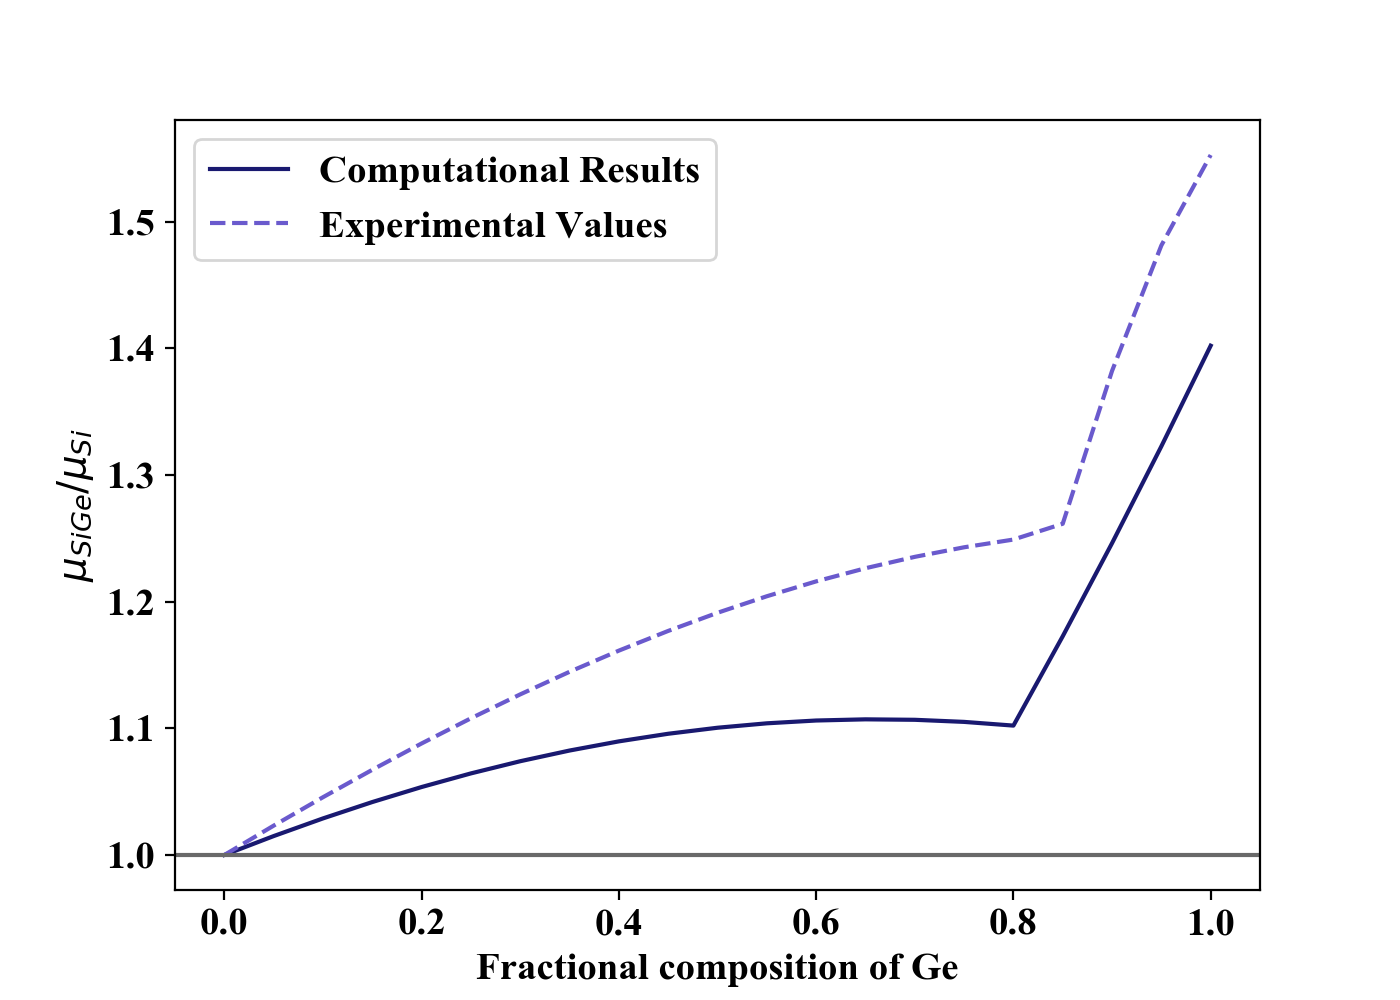
\includegraphics[width=260pt,height=190pt]{ugh.png}

    \caption{Rough trend between the mobility of charge carrier and the composition of germanium.  Note that the y-axis is scaled to some arbitrary constant.}
\end{figure}

We acknowledge that this is a remedial calculation, but serves to illustrate the microscopic argument of the improved mobility of electrons in germanium as compared to silicon. This can be expounded upon in future work.


\subsection{Applications of Charge Carrying Properties}

The band structure shows that germanium has a higher degeneracy of states and  smaller band gap. In comparison with silicon we can conclude that germanium is a better conductor. Mixing of the two results in greater flexibility in the properties of the compounds of SiGe. SiGe compounds are often used in bipolar transistors due to their response time. These often use a smaller percentage of germanium, which will still improve mobility without decreasing the band gap too drastically \cite{ref19}.

Modern techniques of producing SiGe favour the low energy method of layering the compound \cite{ref20} \cite{ref21}. As Vegard's law assumes whole mixing (as in bulk compound), methods of calculating the properties would have to adapt to change the probability of interaction with each ion.

\subsection{Difficulty Modelling Germanium}

Similar discrepancies in the trend for the band gap and effective mass are reported by Rieger \& Vogl \cite{ref07}. The error most likely arises in the interpolation of the form factors. This is due to a crystal disorder present in physical SiGe that fails to be modelled by the simulation. The relationship between these factors is non-linear and cannot be corrected simply with a bowing parameter \cite{ref07}. Production of SiGe is more economic when done at low temperatures. This results in  slight distortions that changes the structure of the crystal to become tetragonal. \\

Another source of error is  due to the inaccuracy of the pseudopotential form factors. The method of generating the form factors is more situational to the method used to obtaining the band structure. This is evident in the discrepancy in the value for the band gap of germanium at 300 K. Most sources site this to be somewhere around 0.66 eV \cite{ref01}, but the methods used here obtained a value of (0.75 $\pm$ 0.03) eV. The reasons for this inaccuracy are not important to this investigation, but this is a valid point against the form factors used. \\



\section{Conclusions \& Future Works}

This work has analysed the usefulness in implementing Vegard's law to potentially linear physical properties of silicon and germanium compounds. The current carrying properties of the compounds as a function of the fraction of germanium were analysed and their physical uses inferred from comparison to their parent compound.\\

The difference in topology and the resulting band gaps were analysed. Where applicable a bowing parameter has been derived and utilised to improve the failings of the linear approximation characteristic of Vegard's law. A decreasing relation similar to that of the sources was inferred. A distinct change in the trend is seen at $x$ = 0.80. \\

The effective mass of electrons in the transverse and longitudinal directions to the conduction band minimum were calculated. From this the values for the conduction electron effective mass are found.  Once again there is a distinct change in the trend at $x$ = 0.80 where the results diverge from literature values. We instead analyse the electron mobility intrinsically.\\

Potential improvements left to future works would be to improve the values for the pseudopotential form factors of germanium. This could be achieved through harder scrutiny of literature values or potentially deriving them specifically for the methods used in this paper.\\

As the shape of the valence band did not vary greatly, the values for the effective mass of the holes has not been discussed. With more time this paper could look into the changes of the properties of these charge carriers in tandem with that of electrons. A broader description of the charge carrying properties could also be given with the density of states described, as this would allow us to explore the effective mass of the density of states. We could continue to analyse whether or not the model breaks down in the germanium-like regime and try to infer a pattern in the errors given. This information would also allow us to make more formal attempt at comparing the electron mobility in the compounds and hence provide a better explanation of the current carrying properties of SiGe compounds.



 \begin{acknowledgements}
 The author would like to thank Dr Christina Zambon for her support in ensuring that this assignment was completed to the best of the author's ability.
 \end{acknowledgements}


\begin{thebibliography}{}

\bibitem{ref01}C. Kittel, Introduction to Solid State Physics 8, Hoboken, NJ, Wiley.  (2004)   % example reference

\bibitem{ref02}T. Luong, V. Thanh, A. Ghrib, M. Kurdi and P. Boucaud, Advances in Natural Sciences, Vol. 6, No. 1. (2015)

\bibitem{ref03}M. Schultze et al., Science, Vol. 346, No. 6215, pp. 1348-1352. (2014)

\bibitem{ref04}M. E. Levinshtein, L. Sergey, L. Rumyantsev, M. Shur. New York: Wiley, (2001)

\bibitem{ref05}E. Kasper, A. Schuh, G. Bauer, B. Hollander, H. Kibbel, Journal of Crystal Growth,
Vol. 157, Iss 1–4, pp. 68-72. (1995)

\bibitem{ref06}L. Vegard, Physik, Vol. 5, pp. 17–26. (1921)

\bibitem{ref07}M. M.  Rieger, P. Vogl, Phys. Rev. B, Vol. 48, Iss. 19, pp. 14276-14287. (1993)

\bibitem{ref08}M. N. Srnec, S. Upadhyay, J. D.  Madura, J. Chem. Educ. 12, Vol. 93, pp.2106-2109. (2016)

\bibitem{ref09}J. Phillips, L. Kleinman, Phys. Rev., Vol. 116, No. 2, pp. 287-294. (1959)

\bibitem{ref10}J. Loehr, Physics of Strained Quantum Well Lasers. New York, NY: Springer. (2013)

\bibitem{ref11}M. Cohen, T. Bergstresser, Phys. Rev., Vol. 141, No. 2, pp. 789-796. (1966)

\bibitem{ref12}J. Weber, M. Alonso, Phys. Rev. B., Vol. 40, No. 8, pp. 5683-5693. (1989)

\bibitem{ref13}E. Barbagiovanni, D. Lockwood, P. Simpson, L. Goncharova, Ap. Phys. Rev. Vol. 1, No. 1. (2014)

\bibitem{ref14}T. Cheema, Higher-order finite-difference methods for partial differential equations. Brunel University. (1997)

\bibitem{ref15}S. Krishnamurthy, A. Sher, A. Chen, Phys. Rev. B, Vol. 33, No. 2, pp. 1026-1035. (1986)

\bibitem{ref16}S. Datta et al., Journal of Physics: Condensed Matter, Vol. 31, No. 49. (2019)

\bibitem{ref17}L. Saravia and D. Brust, Phys. Rev., Vol. 176, No. 3, pp. 915-923. (1968)

\bibitem{ref18}S. Krishnamurthy, A. Sher and A. Chen, Applied Physics Letters, Vol. 47, No. 2, pp. 160-162. (1985)

\bibitem{ref19}Y. M. Haddara, P. Ashburn, D. M. Bagnall, Silicon-Germanium: Properties, Growth and Applications, Springer International Publishing. (2017)

\bibitem{ref20}N. Kennedy et al., J. Appl. Phys., Vol. 126, No. 2. (2019).

\bibitem{ref21}M. Matsuura, J. Tonnerre, G. Cargill, Phys. Rev. B, Vol. 44, No. 8, pp. 3842-3849. (1991)
\end{thebibliography}


\end{document}
